%# -*- coding: utf-8-unix -*-

\chapter{客户端SDK设计与实现}
\label{chap:client}

\section{客户端SDK概要}
\label{sec:clientSDKOverview}

Appetizer客户端SDK是提供给开发者用于集成到App的部分,是达成用户使用App信息收集任务的必要程序。客户端SDK提供给开发者的形式是一个jar包,开发者通过在原来的应用程序代码中插入jar包提供的API达到实现信息收集的目的。

客户端SDK的主要功能包括

 \begin{itemize}
 	\item 用户Session信息收集
 	\item 用户浏览路径和时长信息收集
 	\item 应用崩溃信息和发生崩溃时设备状态收集
 	\item 应用ANR侦测和发生ANR时设备状态收集
 	\item 应用启动黑白屏时间信息收集
 \end{itemize}
 
Appetizer客户端SDK的设计目标是在达到完成需求功能的前提下。为了使jar包占用空间尽可能小,客户端SDK的实现没有使用任何第三方库。为了减少Android应用程序因为集成Appetizer客户端SDK造成的额外性能开销和内存开销,客户端SDK不会启动任何新的进程,所有任务都在原有的Android应用程序进程中实现,包括收集数据、存储数据、发送数据。本章后续几节从设计到实现都体现了Appetizer客户端SDK“轻量级”的目标。
 
Appetizer客户端SDK需要持久化存储的数据都在每个Android应用程序的独立存储区域中,一台Android设备安装了多个集成Appetizer客户端SDK的应用程序,它们的数据不会发生冲突。

设备的本地时间是不可信的,但是Appetizer客户端SDK中记录的时间相关信息只能使用设备本地时间,因此在每个发送到服务端的信息中会加入发送时刻的设备本地时间,服务端可以根据这个时间和服务端本地时间对所有数据的时间进行校准。

\section{客户端SDK架构}
\label{sec:clientSDKArch}

\begin{figure}[!htp]
	\centering
	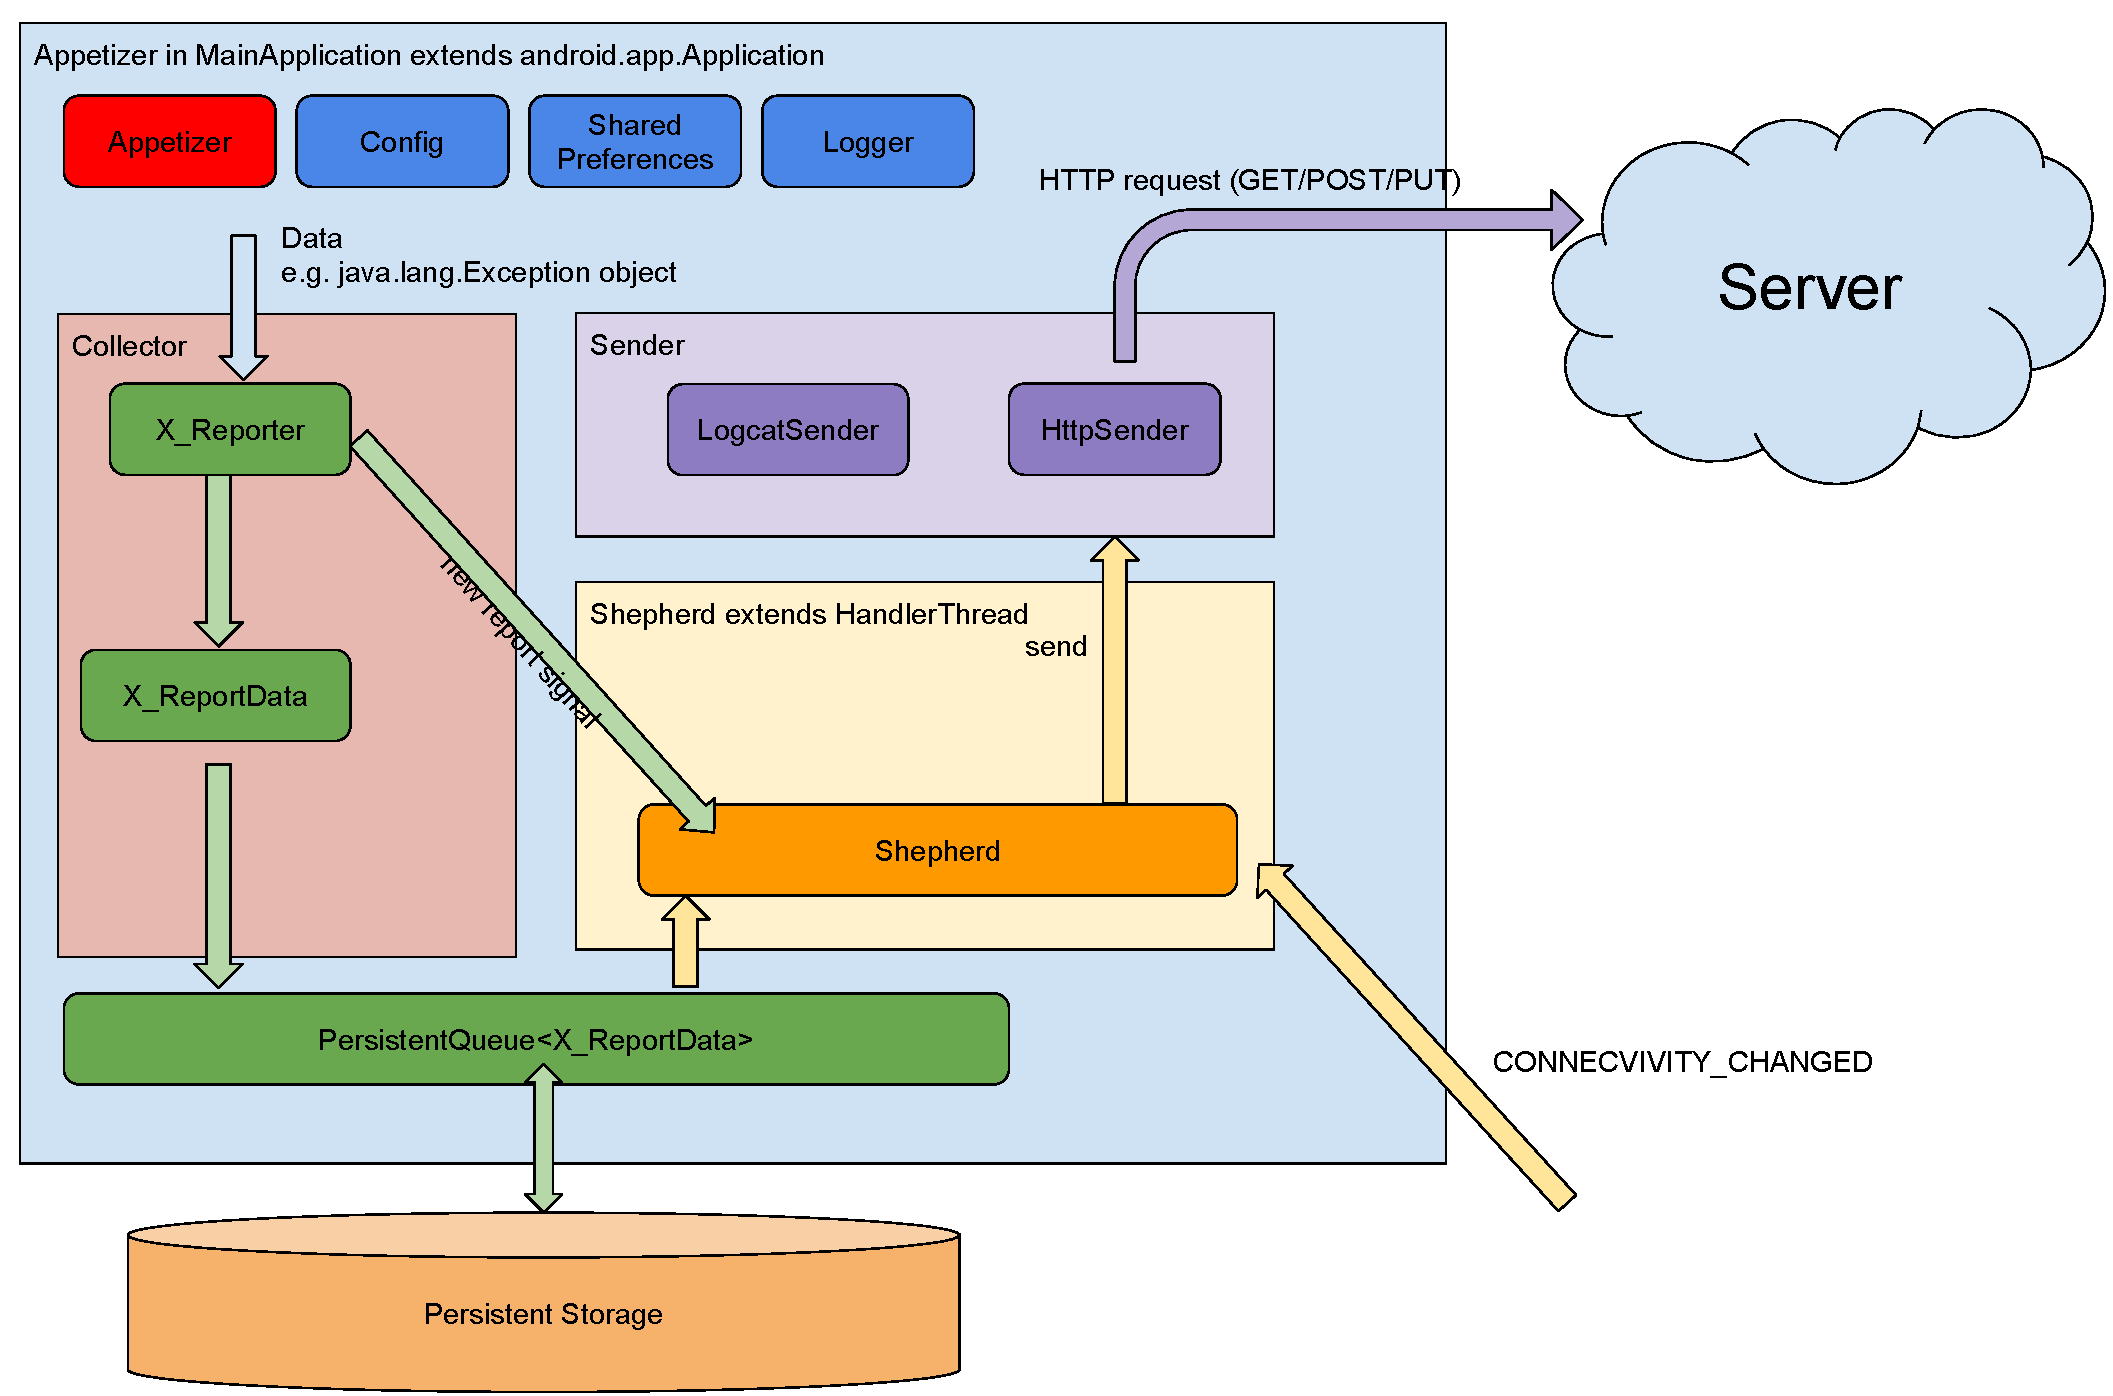
\includegraphics[width=1\textwidth]{client_architecture.pdf}
	\bicaption[fig:clientArchitecture]{这里将出现在插图索引中}{客户端SDK架构}{Fig}{Client SDK architecture}
\end{figure}

客户端SDK主体流程部分架构如图\ref{fig:clientArchitecture}所示,Appetizer客户端SDK的入口类名是“Appetizer”,在Android应用程序的Application类初始化的同时进行初始化,不会创建任何新的进程。Appetizer会读取配置文件,创建自定义的Logger对象,以及使用SharedPreferences访问该Android应用程序与其他应用程序隔离的独立存储空间。

所有需要收集的信息会通过特定的方式传递给Collector,各个信息收集的具体实现方式参见\ref{sec:clientSDKimplement}节。Collector会把收集到的数据存入持久化消息队列,该队列实现的类名为PersistentQueue,实现了Java队列类的全部接口,提供给上层的抽象是程序关闭后,重新运行程序后队列的数据能够恢复,不会丢失,该轻量级持久化消息队列的具体实现参见\ref{subsec:persistentQueue}小节。

Appetizer会在Android应用程序的主进程中创建一个HandlerThread,称为Shepherd,这是一个长时间存在的线程,当有任务需要执行的时候才会被唤醒,避免了一般线程多次销毁创建的开销。Shepherd的作用是判断网络状况,发送持久化消息队列中的数据到服务端。当Collector收到新的数据,会向Shepherd发送消息,Shepherd得到消息会首先判断网络状况,网络状况允许的情况下再将持久化消息队列中积存的消息通过HTTP请求发送给服务端。除此之外,Shepherd注册侦听设备的网络变化状况,当Android设备从未连接到连接互联网成功时,系统会发送网络状况变化的事件消息给所有注册侦听该事件的进程,接收到该消息后Shepherd同样会发送持久化消息中积存的消息给服务端。

\section{客户端SDK实现}
\label{sec:clientSDKimplement}

Appetizer客户端SDK最低支持Android API 9,即Android 2.3 Gingerbread。根据Google官方的数据,截止2016年5月2日,系统版本低于Android 2.3版本的活跃设备数量不足全部活跃设备数量的0.1\%,可以认为Appetizer客户端SDK支持99.9\%以上的Android设备。

\subsection{网络模块}
\label{subsec:networkModulo}

图\ref{fig:clientArchitecture}中的HttpSender模块,即客户端SDK的网络发送部分,该模块基于Apache HTTP Client封装实现,用于将Appetizer客户端SDK收集到的数据通过HTTP POST发送到服务端。

在Android 6.0及以上的系统中,Apache HTTP Client已被弃用,采用Ok HTTP作为默认的HTTP客户端。但是由于Android 6.0及以上的系统使用ART RunTime取代Dalvik虚拟机,ART RunTime不支持在Android应用程序崩溃后创建新线程,Ok HTTP Client发送Http请求后为了不阻塞原线程继续运行,采用创建新线程的方式异步接受服务端的返回值,导致的问题是在ART RunTime下Andorid应用崩溃后无法使用Ok HTTP\parencite{create_thread}。因此Appetizer客户端SDK的网络模块,基于老版本Android系统默认的Apache HTTP Client进行封装实现。

\subsection{持久化队列}
\label{subsec:persistentQueue}

Appetizer客户端SDK的持久化队列PersistentQueue,能够存储任何二进制数据,实现了Java Queue的全部接口,任何Java使用抽象类Queue申明的对象都可以被赋值为PersistentQueue,而且对象的操作方法保持不变。

每次程序对PersistentQueue对象的入队或者出队操作成功后,队列的持久化存储数据都会发生变化。Android应用程序关闭、设备重启或者内存断电后,当Android应用程序重启启动时,Appetizer初始化时能够恢复持久化消息队列到上一次操作成功后的状态。Appetizer客户端SDK实现的持久化队列PersistentQueue基于Android的轻量级key-value存储系统SharedPreferences和Android的文件系统进行实现,并且保证了操作的原子性,在PersistentQueue方法执行的过程中发生了断电、存储硬件被取出等会导致方法无法正常执行或中断的情况时,Appetizer重新初始化后PersistentQueue能够还原到该操作没有进行的状态。

Android的key-value存储系统SharedPreferences底层是基于文件系统和XML格式实现的,并且保证了原子性和一致性。在Appetizer客户端SDK的功能需求上,需要持久化队列保存Java对象序列化后的二进制数据,SharedPreferences通常用于实现配置文件存储,简单的用户信息存储等。但是由于SharedPreferences存储实现的编码问题,不同的编码对于文本换行符的定义不一致,单个字节0x0A通过SharedPreferences写入后再读出会变成字节0x0D,因此无法使用SharedPreferences保存Java序列化对象。一种解决办法是存储Base64编码的对象序列化数据,但是比较复杂的对象序列化数据很大,每次操作进行Base64编码的计算开销过大不能接受。

Android的文件系统可以写入和读取二进制数据,并且数据不会发生变化,但是Android系统提供的文件操作无法保证操作的原子性,如果在文件写入操作执行过程中发生了程序崩溃、设备断电或者存储硬件被取出等问题,会导致只有部分数据成功写入,而且程序无法判断写入操作是否成功执行,因此再进行读取操作时会发生问题。

Appetizer客户端SDK实现的原则是不使用第三方库,对文件系统的操作进行封装,同时支持原子性和Java对象序列化持久存储,比较复杂而且难以保证实现的正确性。结合支持原子性操作的SharedPreferences和支持Java对象序列化持久存储的文件系统操作API,可以通过简单的方式实现日志式解决方案的支持原子性的持久化消息队列。

每个PersistentQueue对象中包括四个成员对象,SharedPreferences句柄、两个文件句柄和存储在内存的LinkedList对象。

创建PersistentQueue对象时会进行初始化,首先从SharedPreferences中读取持久化保存的当前PersistentQueue的状态,获取最后一次成功的原子操作后数据存储的文件,然后调用文件IO API读取文件中的数据流,数据流反序列化成对象赋值给LinkedList对象。如果不存在之前的PersistentQueue存储文件,会创建空的LinkedList对象,再调用原子性文件写入操作。

PersistentQueue的关键技术是原子性文件写入操作,步骤如下:

\begin{enumerate}
	\item 读取SharedPreferences的状态信息,获取当前数据保存的文件,选择写入另一个文件。
	\item SharedPreferences的状态改变为“文件写入操作开始”。
	\item 序列化LinkedList对象并写入文件流。
	\item SharedPreferences的状态改变为“文件写入操作完成”。
\end{enumerate} 

如果操作在第1步崩溃,因为没有开始写入操作,重新载入不会出现问题。操作第2、4步由SharedPreferences保证原子性。如果在操作第3步崩溃,重新载入恢复的时候根据SharedPreferences的状态信息判断在文件写入时崩溃,读取另一个文件反序列化恢复LinkedList对象数据。图\ref{fig:persistentQueue}展现了Appetizer操作持久化队列的程序执行流程,其中File A和File B互为备份,交替写入,状态都保存在SharedPreferences中。

\begin{figure}[!htp]
	\centering
	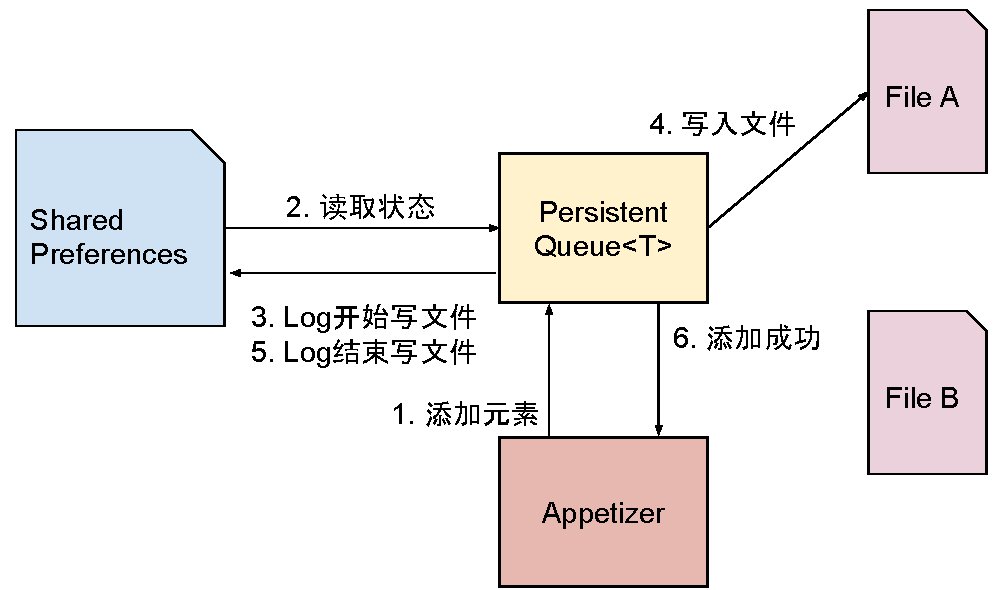
\includegraphics[width=1.0\textwidth]{persistentQueue.pdf}
	\bicaption[fig:persistentQueue]{这里将出现在插图索引中}{持久化队列}{Fig}{Persistent Queue}
\end{figure}

PersistentQueue的单个元素修改、增加、删除操作,首先操作LinkedList的元素,然后调用原子性文件写入操作保证数据持久化存储,最后函数执行完成,返回函数返回值。PersistentQueue的多个元素操作为了提高性能避免多次原子性文件写入操作,在对内存中的LinkedList对象修改全部执行完毕后调用一次原子性文件写入操作,而不是简单的复用单个元素的修改进行实现。

PersistentQueue的元素读取操作直接读取内存中的LinkedList对象,不需要其他的修改。

在Appetizer客户端SDK的实现中,存在三个PersistentQueue对象,分别是用户会话信息的持久化队列、崩溃信息和ANR信息的持久化队列、黑白屏时长信息的持久化队列,其中ANR信息和崩溃信息收集的数据类似,因此合并成一个数据类,共用同一个持久化队列。

\subsection{用户会话收集}
\label{subsec:sessionCollector}

用户使用Android应用的会话信息(App session)是所有信息收集功能中被调用最频繁的一个,Android应用程序的浏览“页面”被定义为每个Activity和Fragment,因此当用户每次切换“界面”的时候都需要收集信息。Appetizer客户端SDK收集的浏览路径时间,定义为从Activity和Fragment生命周期的onResume开始,到onPause结束。
在每个开发者想做数据收集的Activity和Fragment的这两个生命周期函数开头,需要插入一行代码调用Appetizer客户端SDK提供的API,并将this(Context对象)作为参数传入。用户会话信息的时间全部使用从epoch开始的时间戳表示,单位毫秒。

因为在Android系统中,每个进程被杀死的时候进程本身不能再执行任何操作,无法在强制退出前保存状态,因此为了在Android应用程序进程被强制杀死的时候用户会话信息不丢失,在一个会话里每次浏览路径更新的时候需要持久化存储会话当前的快照。
快照更新事件的频率较高,如果快照通过PersistentQueue进行持久化存储,开销过大。
用户会话信息包括浏览路径可以通过字符串表示,因此不需要进行序列化存储在PersistentQueue中,可以使用SharedPreferences完成快照持久化存储的目的。

Android应用程序正常使用并正常退出的情况下,用户会话信息变化如下:

\begin{enumerate}
	\item Android应用程序启动,内存中创建新的session对象,并写入会话开始时间和浏览路径节点开始时间和节点名,当前会话快照存入SharedPreferences。
	\item 用户切换“界面”,session对象写入上个浏览路径节点的结束时间,判断上个节点浏览时间是否超过30秒,如果未超过则写入新的浏览路径节点的开始时间,如果超过30秒则将上个session对象存入PersistentQueue,创建新的session对象,并写入会话开始时间和浏览路径节点开始时间和节点名,当前会话快照存入SharedPreferences。该步骤循环零次或者若干次。
	\item 用户将该Android应用程序退到后台,session对象写入当前浏览路径节点的结束时间,当前会话快照存入SharedPreferences。
	\item 用户将该Android应用程序从后台切换到前台,判断距离上个节点浏览结束的时刻是否超过30秒,如果未超过则写入新的浏览路径节点的开始时间,如果超过30秒则将上个session对象存入PersistentQueue,创建新的session对象,并写入会话开始时间和浏览路径节点开始时间和节点名,当前会话快照存入SharedPreferences。
\end{enumerate} 

在很多情况下Android应用程序会被强制杀死,例如系统内存不足的时候,系统会决定杀死部分进程释放内存,或者内存清理工具、安全管家等软件会将进程杀死。在进程被杀死后,用户会话信息只存储在SharedPreferences里,并没有作为一个完整的会话数据加入持久化消息队列中。Appetizer客户端SDK考虑到了这种情况,在该Android应用程序下次启动的时候,用户会话收集的Collector实例初始化阶段会从SharedPreferences里恢复应用程序被杀死前的用户会话快照,写入持久化消息队列并清除快照。

\subsection{崩溃信息收集}
\label{subsec:crashCollector}

崩溃信息收集是Appetizer客户端SDK的重要功能,开发者只需要在应用程序的Application调用Appetizer的初始化方法,就自动集成好了崩溃信息收集功能。

崩溃信息收集功能的核心部分是单例类CrashReporter,在Appetizer初始化的时候创建。CrashReporter继承了接口Thread.UncaughtExceptionHandler,实现了uncaughtException方法,并调用Android SDK方法Thread.setDefaultUncaughtExceptionHandler传入自身作为参数,把CrashReporter设置为默认的异常处理类,可以捕获全局异常。
所有未被捕获的异常都会导致Android应用崩溃,如果设置了全局异常捕获,在应用发生崩溃前异常会被CrashReport的uncaughtException方法捕获,可以在该方法内实现崩溃信息和设备实时状态信息的收集。

在uncaughtException方法中,首先保存用户会话信息到持久化消息队列,因为此时Android应用程序发生崩溃,本次会话结束。然后读取异常、线程和设备状态的数据,收集需要的信息加入持久化消息队列,并发送信号到Shepherd触发网络发送事件。崩溃时收集的数据如下:

 \begin{itemize}
 	\item 设备国际移动设备标识(IMEI),15位数字字符串,例如“358239058889108”。
 	\item 应用版本名(App version name),字符串数据,例如“2.1.1 Alpha”。
 	\item 应用版本号(App version code),数值数据,例如“10”。
 	\item 应用包名(App version name),字符串数据,例如“io.appetizer.demo”。
 	\item 文件路径(File path),例如“/data/user/0/io.appetizer.demo/files”。
 	\item 设备型号(Phone model),例如“Nexus 5”。
 	\item 设备品牌 (Brand),例如“google”。
 	\item 产品名 (Product),例如“hammerhead”。
 	\item 系统版本(Android system version),例如“6.0”。
 	\item 系统构建数据 (Android build information),包含了系统ROM的详细信息。
 	\item 内存总大小和内存剩余大小(RAM size),内存剩余大小指崩溃时的设备内存剩余大小。
 	\item 闪存总大小和闪存剩余大小(Flash size),通常是手机内不可取出的存储硬件。
 	\item 外部总大小和外部剩余大小(External size),通常是手机内可取出的存储卡。
 	\item 函数调用栈(Stack trace),Exception对象有价值的数据转为JSON格式发送,格式化的数据方便服务端分析,没有信息丢失。
 	\item 函数调用栈哈希值(Stack trace hash),用于快速查找合并相同的崩溃原因。
 	\item 应用启动时设备设置信息(Initial configuration),包括字体大小、音量大小等。
 	\item 应用崩溃时设备设置信息(Crash configuration),具体内容同上。
 	\item 屏幕信息,包括屏幕尺寸、分辨率等。
 	\item 设备硬件支持列表(Device features),显示设备支持的功能,包括蓝牙、相机、多点触控、GPS、NFC等。
 	\item 网络信息(IP),设备崩溃时的网络环境信息和IP地址。
 \end{itemize}
 
 上述收集的崩溃数据以Java序列化对象的形式存储在持久化消息队列中,当Shepherd判断网络可以发送时,反序列化消息队列的崩溃信息,再转为JSON格式放入HTTP POST body中发送到服务端。崩溃信息数据量庞大,转为JSON格式开销较大,但是相比于用户会话,崩溃信息收集事件发生的频率较低,因此格式转换的开销影响不大。
 
 崩溃时收集的部分信息设计到读取设备敏感信息,需要额外的权限,Appetizer客户端SDK需要Android应用程序提供的权限原由来自于此。包括:
 
\begin{itemize}
 	\item android.permission.READ\_PHONE\_STATE
 	\item android.permission.ACCESS\_NETWORK\_STATE
 	\item android.permission.ACCESS\_WIFI\_STATE
\end{itemize}

如果开发者的应用程序源代码中的Manifest没有申明这些权限,Appetizer客户端SDK的崩溃信息收集功能会有部分数据无法收集。

\subsection{ANR侦测}
\label{subsec:ANRCollector}

\begin{figure}[!htp]
	\centering
	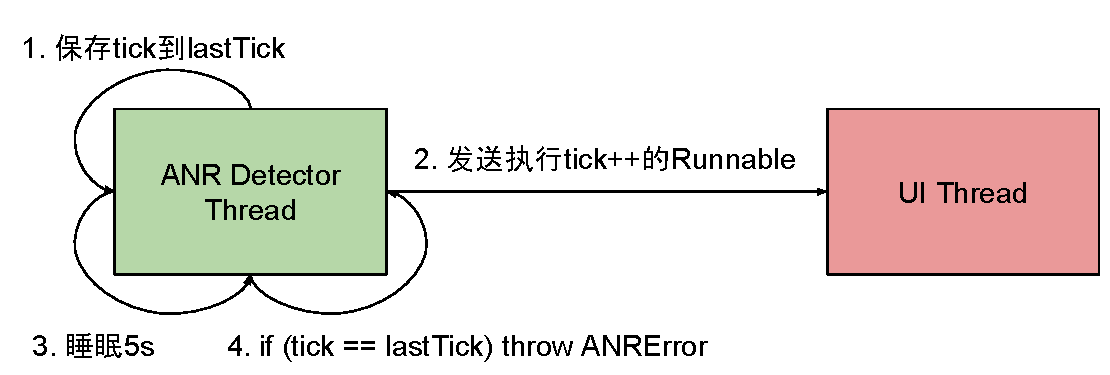
\includegraphics[width=1.0\textwidth]{ANR.pdf}
	\bicaption[fig:ANR]{这里将出现在插图索引中}{ANR侦测流程}{Fig}{ANR detector workflow}
\end{figure}

\ref{subsec:background_ANR}小节介绍了Android应用程序未响应(ANR)的相关背景知识,Appetizer客户端SDK的ANR侦测参考了ANR-WatchDog\parencite{watchdog}并复用崩溃信息收集功能,在实现上进行了一定程度的简化。

集成了ANR侦测功能的Android应用程序在前台运行时,ANR侦测功能开启。ANR侦测模块会创建volatile整形数值变量tick,并在Android应用程序主进程中创建一个新的线程,volatile关键字会保证一个线程更新了某个对象后会立刻同步到其他线程,不会因为线程变量缓存的问题造成数据同步延迟问题,如图\ref{fig:ANR}所示,ANR侦测线程会保存当前tick的数值到lastTick变量,再发送一个会对tick进行加一操作的Runnable给主线程(UI线程)执行,volatile关键字的存在保证了主线程更新tick之后ANR侦测线程可以获取到最新的tick的值,然后睡眠5秒检查tick和lastTick变量是否相同。
如果数值相同,则说明主线程在5秒内没有空余时间执行发送过去的Runnable,认为此时主线程发生应用程序未响应,ANR侦测程序会创建ANRError对象,ANRError继承Java Error类并且能够收集所有线程的函数调用栈,ANR侦测程序再抛出ANRError对象,\ref{subsec:crashCollector}小节描述的应用崩溃信息收集模块会捕获该错误,并按照发生崩溃的流程收集此时的设备状态信息,ANRError错误中包含了此时所有线程函数调用栈信息,方便开发者进行应用程序未响应错误原因的定位。通过抛出ANRError的操作复用了应用程序崩溃信息收集模块,避免单独开发,减少Appetizer客户端SDK的占用空间,并且可以和一般的应用程序崩溃信息共用一个持久化消息队列。
如果数值不同,则说明主线程在5秒内执行了发送过去的Runnable,可以认为过去的5秒主线程没有发生应用程序未响应的问题,该ANR侦测线程继续保存tick到lastTick,发送Runnable并睡眠5秒,如此循环。

如果ANR侦测线程不间断运行,会导致设备的处理器无法休眠,耗电量增大。为了减少ANR侦测的开销,Appetizer客户端SDK注册侦听设备屏幕关闭事件,当Android应用程序切换到后台或者设备屏幕关闭,ANR侦测线程会长时间休眠,当该Android应用程序切换到前台使用时ANR侦测模块才会重新开启。ANR侦测程序的逻辑代码计算量不大,而且每5秒执行一次,对Android应用程序造成的性能影响不大。

\subsection{黑白屏时长记录}
\label{subsec:blackWhiteCollector}

黑白屏时长是指Android应用程序启动后到加载第一个页面完成之间的时间,在Android Activity生命周期中是从onCreate开始到onResume这一段时间。因此开发者在Android应用程序中启动后的第一个Activity的onCreate开头和onResume结束调用Appetizer客户端SDK提供的两个API,就能够记录Android应用启动时黑白屏时长。Appetizer客户端SDK的这两个API会记录被调用时设备的本地时间,加入到持久化消息队列等待发送到服务端。本地时间是不可信的,但是黑白屏记录的两个时间点间隔较小,而且只需要两个时间点的时间差,因此两个本地时间点的差值可以直接作为可信的黑白屏时长数据。

\section{本章小结}

本章内容篇幅较大,介绍了Appetizer客户端SDK的方方面面,是整个项目技术实现的核心部分。

\ref{sec:clientSDKOverview}节介绍了Appetizer客户端SDK的主要功能、轻量级的特点、多个应用数据隔离和对不可信的本地时间校准的方法。

\ref{sec:clientSDKArch}节通过架构图从宏观上介绍了Appetizer客户端SDK的各个模块的作用和各个模块之间的关联。

\ref{sec:clientSDKimplement}节详细介绍了Appetizer客户端SDK各个功能模块的设计方案、取舍原因和实现过程。
\ref{subsec:networkModulo}小节介绍了选择Apache HTTP客户端的原因。
\ref{subsec:persistentQueue}小节介绍了实现持久化消息队列的重要性,选择基于SharedPreferences和Android文件系统实现持久化消息队列的原因,以及持久化消息队列原子性的实现细节和使用方法,比较深入详细。
\ref{subsec:sessionCollector}小节介绍了用户会话的定义,在Android系统下用户会话信息收集的难点,以及通过结合SharedPreferences、快照和持久化消息队列的解决方法,用户会话信息收集是Appetizer客户端SDK的核心功能之一。
\ref{subsec:crashCollector}小节介绍了崩溃信息收集模块,主要包括崩溃时收集数据的方法,数据的具体内容和需要的系统权限,崩溃信息收集也是Appetizer客户端SDK的核心功能之一。
\ref{subsec:ANRCollector}小节介绍了Appetizer客户端SDK实现Android应用程序未响应侦测的方法,还分析了该功能对Android应用程序性能的影响。
\ref{subsec:blackWhiteCollector}小节介绍了黑白屏时长记录的实现方法和向开发者提供的API的用法。